\documentclass{report}
\usepackage{amsmath}
\usepackage{amsfonts}
\usepackage{hyperref}
\usepackage[english,russian]{babel}
\usepackage{graphicx}


\DeclareMathOperator{\grad}{grad}
\newcommand{\divg}{\mathrm{div}\,}

\begin{document}
	
\section{Постановка задачи}
Решается двумерная задача Дирихле для двумерного стационарного оператора диффузии

$$
\begin{cases}
    \divg(-\mathbb{D} \grad u) = f, x \in \Omega, \\
    u|_{\partial \Omega} = g.
\end{cases}
$$
$
    \Omega = [0,1]^2, D = diag(d_x, d_y).
$

Задача решается методом конечных разностей на регулярной квадратной сетке
\[
    w_h = {ih, jh}, h = \frac{1}{N}
\]
с помощью пятиточечного шаблона
\[
    \frac{\partial^2 u}{\partial x^2}(x_i, y_j) \equiv \frac{u^h_{i+1,j} - 2u^h_{i,j} + u^h_{i-1,j}}{h^2},
\]
\[
    \frac{\partial^2 u}{\partial y^2}(x_i, y_j) \equiv \frac{u^h_{i,j+1} - 2u^h_{i,j} + u^h_{i,j-1}}{h^2},
\].

Полученная система решается с помощью библиотеки \href{https://github.com/INMOST-DEV/INMOST}{INMOST}.


\section{Численный эксперимент}

Эксперимент проводился для задач, в которых известно аналитическое решение, а именно
\begin{enumerate}
	\item $f = \sin(\pi x) \sin(\pi y),~ g = 0, d_x = d_y = 1$. $u = \frac{\sin(\pi x) \sin(\pi y)}{2 \pi^2}$.
	\item $f = \sin(10 x) \sin(10 y), ~ g = \frac{\sin(10 x) \sin(10 y)}{200} , d_x = d_y = 1$. $u = \frac{\sin(10 x) \sin(10 y)}{200}$.
	\item $f = \sin(4 \pi x) \sin(\pi y), ~ g = 0, d_x = 5, d_y = 1$. $u = \frac{\sin(4 \pi x) \sin(\pi y)}{(16d_x + d_y)\pi^2}$.
\end{enumerate}

Для всех трех экспрементов построены графики С-нормы и среднего значение среднекваратичного отклонения при сгущении сетки.
Для второго эксперимента также построено само решение.

\begin{figure}[!h]
	\centering
	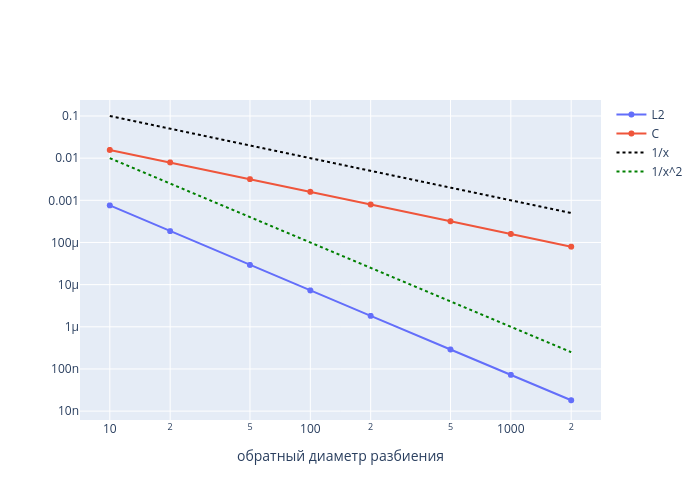
\includegraphics[width=0.9\textwidth]{img/pixpiy.png}
	\caption{$f = \sin(\pi x) \sin(\pi y),~ g = 0, d_x = d_y = 1$}
\end{figure}

\begin{figure}[!h]
	\centering
	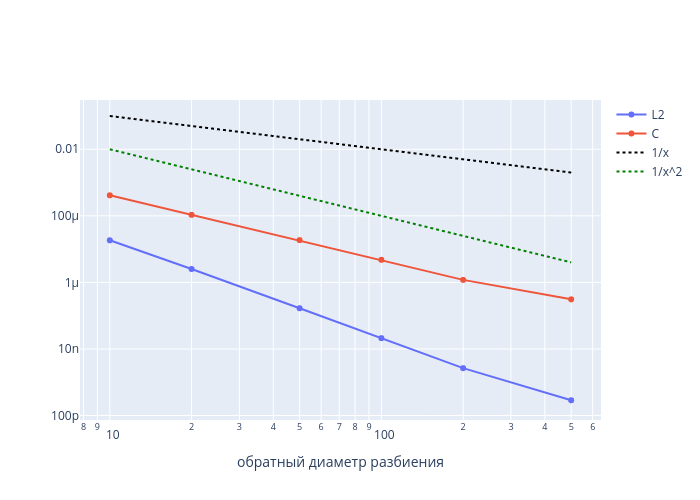
\includegraphics[width=0.9\textwidth]{img/10x10y.png}
	\caption{$f = \sin(10 x) \sin(10 y), ~ g = \frac{\sin(10 x) \sin(10 y)}{200} , d_x = d_y = 1$}
\end{figure}

\begin{figure}[!h]
	\centering
	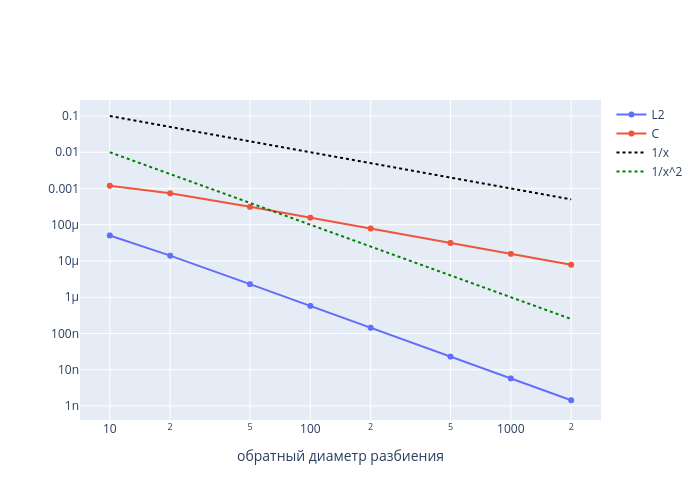
\includegraphics[width=0.9\textwidth]{img/4pixpiy.png}
	\caption{ $f = \sin(4 \pi x) \sin(\pi y), ~ g = 0, d_x = 5, d_y = 1$}
\end{figure}


\begin{figure}[!htb]
	\minipage{0.33\textwidth}
	\includegraphics[width=\textwidth]{img/10.png}
	\caption{$u, N = 10$}
	\endminipage\hfill
	\minipage{0.33\textwidth}
	\includegraphics[width=\textwidth]{img/100.png}
	\caption{$u, N = 100$}
	\endminipage\hfill
	\minipage{0.33\textwidth}%
	\includegraphics[width=\textwidth]{img/1000.png}
	\caption{$u, N = 1000$}
	\endminipage
\end{figure}

\end{document}